\documentclass[11pt]{article}

\usepackage[letterpaper,margin=1in]{geometry}
\usepackage{amsmath,amssymb}
\usepackage{booktabs}
\usepackage{array}
\usepackage{graphicx}
\usepackage{caption}
\usepackage{listings}
\usepackage{enumitem}
\usepackage{xcolor}
\usepackage[colorlinks=true,linkcolor=blue,urlcolor=blue]{hyperref}

\setlength{\parindent}{1.5em}
\setlength{\parskip}{0pt}
\setlength{\emergencystretch}{2em}
\renewcommand{\arraystretch}{1.15}
\captionsetup{skip=4pt}

\title{\vspace{-2em}EE180 Project 1: Biomedical Signal Processing\\\large Spinal Tissue Classification from Ultrasound Signals}
\author{Renyi Yang \qquad 2023533030}
\date{}

\begin{document}
\maketitle

\section{Introduction}

Accurate identification of spinal tissues during ultrasound-guided procedures is
important for surgical safety, yet the classification of tissue types from
ultrasound backscatter is challenging because the four tissues considered here
(spinal cord, nucleus pulposus, adipose tissue, and nerve root) produce
qualitatively similar echo patterns. This project investigates a complete
classification pipeline for ultrasound signals recorded from sheep spines:
signal preprocessing, adaptive feature extraction, an interpretable statistical
classification rule, general-purpose machine learning classifiers, and a
Vision-Transformer (ViT) baseline.

\section{Data and Preprocessing}

The dataset contains ultrasound signals from a 16-element transducer; every
three consecutive elements form one beam, so each biological sample provides
14 signals of 896 sampling points acquired at $f_s = 75$~MHz. Labels are
0 (spinal cord), 1 (nucleus pulposus), 2 (adipose tissue), and 5 (nerve root).
The released split contains 506 training, 126 validation, and 126 test
biological samples (7{,}084 / 1{,}764 / 1{,}764 signals). Class distributions
are imbalanced, with adipose tissue being the smallest class
(73/18/18 samples in train/val/test).

Because amplitudes are stored as integers in $[0,255]$ around a DC offset of
127.5, samples exactly at the offset may appear as either 127 or 128. All values
equal to 127 or 128 were replaced by 127.5, and each signal was normalized as
\begin{equation}
    x_{\mathrm{norm}}[n]=\frac{x_{\mathrm{us}}[n]-127.5}{127.5}\,\in[-1,1].
\end{equation}
Roughly 60--70\% of the samples of a typical signal lie on this DC baseline,
so the preprocessing mainly removes a quantization artifact of the acquisition
hardware before any spectral analysis. The 14 signals of one biological sample
were kept together in every experiment (five-fold cross-validation folds,
training, and evaluation) to prevent leakage between signals of the same
specimen.

\section{Feature Extraction}

We adopt the Discrete Wavelet Transform (DWT) with Daubechies-4 wavelets
(\texttt{db4}) at decomposition level 5, applied to the preprocessed signals.
The DWT was preferred over EWT because it provides a fixed, well-understood
time--frequency tiling with no per-signal parameter estimation and pywt's
implementation is deterministic and fast; the level-5 decomposition splits the
$0$--$37.5$~MHz band into six sub-bands with approximately octave spacing
(cD1: 18.75--37.5~MHz, \dots, cA5: 0--1.17~MHz), which covers both the
high-frequency scatterer-related content and the low-frequency envelope
structure observed in these signals.

For each of the six components (cA5, cD5, \dots, cD1) we compute the six
required statistics: mean, variance, median, kurtosis, RMS, and skewness,
yielding a 36-dimensional feature vector per signal. Kurtosis and skewness use
SciPy's default biased estimators. A univariate F-test on the training set
shows that the most discriminative features are higher-order statistics of the
finest detail bands, e.g.\ \texttt{cD1\_kurtosis} ($F=1224$),
\texttt{cD2\_rms} ($F=902$), and \texttt{cD2\_kurtosis} ($F=841$). One feature
(\texttt{cD1\_median}) is constant zero because the DC baseline makes the
majority of the finest-scale coefficients exactly zero; it is harmless but
carries no information.

\section{Task 1: Interpretable Statistical Classification Rule}

\subsection{Rule Construction}

The statistical decision rule is a shallow decision tree whose thresholds are
estimated on the training set. A decision tree expresses exactly the type of
criterion the project asks for: an explicit mapping from statistical features
to tissue classes via feature thresholds, without any of the general-purpose
classifiers reserved for Task 2. Candidate rules differ in maximum depth
(3--5) and class weighting (plain or \texttt{balanced} to counter the class
imbalance); the configuration was selected by the same sample-level,
stratified five-fold cross-validation protocol used in Task 2 (Table~\ref{tab:t1cv}).
Signal-level predictions are aggregated per sample by majority voting.

\begin{table}[htbp]
\centering
\caption{Task 1 candidate rules, sample-level cross-validation accuracy
(mean $\pm$ std over five folds). Selection used only the training set;
the validation set is reported afterwards for confirmation.}
\label{tab:t1cv}
\small
\begin{tabular}{lccc}
\toprule
Maximum depth & Class weighting & Sample acc. & std\\
\midrule
3 & plain & 0.7490 & 0.0260\\
3 & balanced & 0.7311 & 0.0304\\
4 & plain & 0.7648 & 0.0229\\
4 & balanced & 0.7904 & 0.0387\\
5 & plain & 0.7984 & 0.0287\\
5 & balanced & \textbf{0.8082} & 0.0339\\
\bottomrule
\end{tabular}
\end{table}

\subsection{Selected Rule}

The selected rule (depth 5 with balanced class weights) is fully reported in
Appendix~\ref{app:rule}: it is a hierarchy of at most five threshold tests on
13 of the 36 features. The root split, \texttt{cD1\_kurtosis} $\le 26.75$,
carves out the low-kurtosis region dominated by nerve-root and adipose echoes;
deeper splits then separate the remaining classes using detail-band RMS and
cD2 statistics. This is
consistent with the per-class statistics in Table~\ref{tab:t1stats}: nerve root
shows markedly lower detail-band kurtosis ($26.4$ for cD1) than nucleus
pulposus ($87.6$), which reflects the sparser, more impulsive high-frequency
content of nerve-root echoes.

\begin{table}[htbp]
\centering
\caption{Training-set statistics (mean) of representative features used by the
rule. Values are dimensionless except RMS (normalized amplitude units).}
\label{tab:t1stats}
\small
\begin{tabular}{lcccc}
\toprule
Feature & Spinal cord & Nucleus pulposus & Adipose & Nerve root\\
\midrule
\texttt{cD1\_kurtosis} & 58.4 & 87.6 & 55.5 & 26.4\\
\texttt{cD2\_kurtosis} & 51.6 & 71.4 & 53.6 & 29.3\\
\texttt{cD2\_rms} & $4.48\times10^{-2}$ & $1.65\times10^{-2}$ & $2.18\times10^{-2}$ & $2.77\times10^{-2}$\\
\texttt{cD5\_skewness} & 0.02 & 2.01 & 1.53 & 0.74\\
\bottomrule
\end{tabular}
\end{table}

\begin{figure}[htbp]
\centering
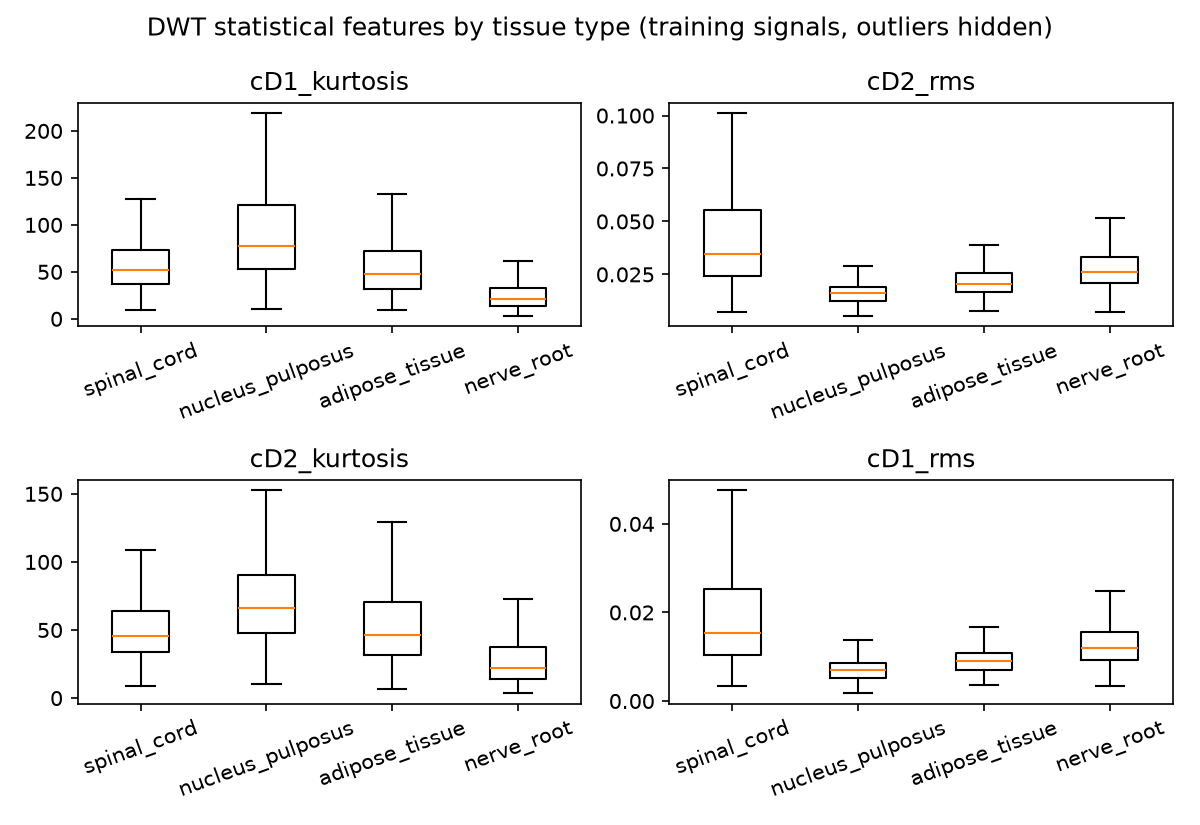
\includegraphics[width=0.78\textwidth]{../code/results/box_task1_features.png}
\caption{Distributions of the four most discriminative rule features across the
four tissue types (training signals, outliers hidden). Spinal cord is
distinguished mainly by detail-band RMS, nucleus pulposus by high kurtosis and
positive low-frequency skewness, and nerve root by low kurtosis.}
\label{fig:box}
\end{figure}

\subsection{Results}

\begin{table}[htbp]
\centering
\caption{Task 1 (statistical rule) results. Accuracy, sensitivity, and
specificity follow the one-versus-rest micro aggregation described in
Appendix~\ref{app:metrics}. ``Signal acc.'' is the accuracy before majority
voting.}
\label{tab:t1res}
\small
\begin{tabular}{lccccc}
\toprule
Split & Accuracy & Sensitivity & Specificity & Signal acc. & no. samples\\
\midrule
Train & 0.8281 & 0.8281 & 0.9427 & 0.6798 & 506\\
Validation & 0.8095 & 0.8095 & 0.9365 & 0.6752 & 126\\
Test & 0.8333 & 0.8333 & 0.9444 & 0.6990 & 126\\
\bottomrule
\end{tabular}
\end{table}

\begin{table}[htbp]
\centering
\caption{Task 1 per-class test metrics (one-versus-rest).}
\label{tab:t1per}
\small
\begin{tabular}{lccccc}
\toprule
Class & Precision & Recall & Specificity & F1 & Support\\
\midrule
Spinal cord & 0.968 & 0.811 & 0.989 & 0.882 & 37\\
Nucleus pulposus & 0.867 & 0.812 & 0.957 & 0.839 & 32\\
Adipose tissue & 0.480 & 0.667 & 0.880 & 0.558 & 18\\
Nerve root & 0.925 & 0.949 & 0.966 & 0.937 & 39\\
\bottomrule
\end{tabular}
\end{table}

\begin{figure}[htbp]
\centering
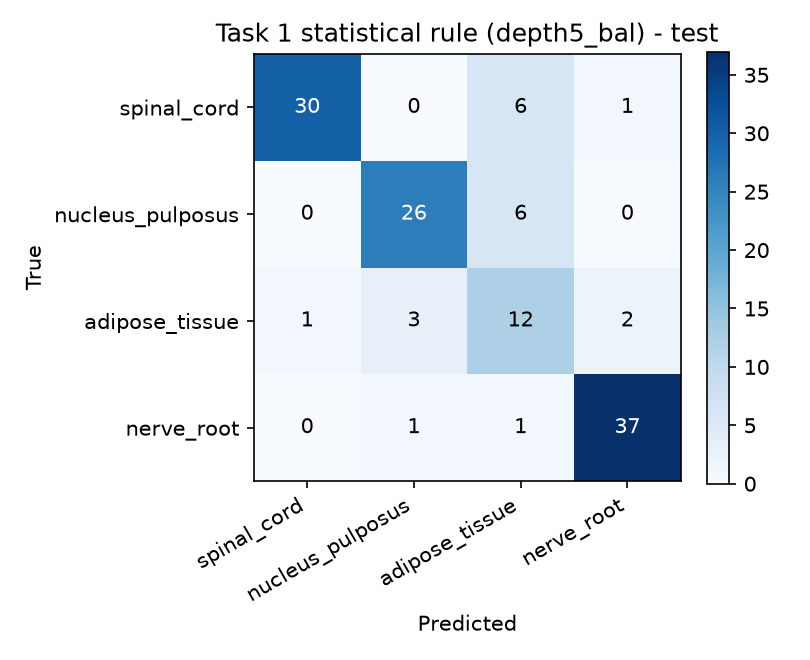
\includegraphics[width=0.46\textwidth]{../code/results/cm_task1_test.png}
\caption{Task 1 confusion matrix on the test set (sample level). The dominant
error is adipose tissue confused with nucleus pulposus and spinal cord.}
\label{fig:cm1}
\end{figure}

The rule reaches $83.3\%$ sample-level accuracy on the test set ($82.8\%$ on
training data, $81.0\%$ on validation), i.e.\ performance is stable across
splits. The per-class metrics show that the errors are concentrated in adipose
tissue (recall $0.67$, precision $0.48$): with only 73 training samples this
class overlaps heavily with the nucleus-pulposus and spinal-cord feature
regions, and the tree cannot afford further splits for it. Nerve root and
spinal cord are classified reliably. The gap between signal-level
($70.0\%$) and sample-level ($83.3\%$) accuracy confirms that majority voting
effectively exploits the consistency of the 14 beams within a sample.

\section{Task 2: Machine Learning Classification}

\subsection{Protocol}

Task 2 uses the same 36 DWT features. Model selection follows the required
protocol strictly:
\begin{itemize}[leftmargin=1.4em,itemsep=1pt]
    \item \textbf{Five-fold cross-validation at the biological-sample level}:
        \texttt{StratifiedGroupKFold} with the sample id as group, so all 14
        signals of a specimen stay in the same fold, and folds are stratified
        over the class distribution.
    \item \textbf{In-fold fitting}: a \texttt{StandardScaler} is fitted only on
        the training part of each fold and then applied to the held-out part;
        no data-dependent quantity crosses fold boundaries.
    \item \textbf{Hyperparameters considered}: SVM (RBF) $C \in \{1, 10, 100\}$
        and class-weighted SVM ($C=10$); random forest (300 trees) with and
        without class balancing; $k$-NN with $k \in \{5, 15, 45\}$.
    \item \textbf{Selection criterion}: mean sample-level accuracy across the
        five folds (majority vote per sample, ties broken by the largest mean
        decision value). The winner is retrained on the full training set;
        validation confirms it, and the test set is evaluated once, after all
        decisions are frozen.
\end{itemize}

\subsection{Cross-Validation Results}

\begin{table}[htbp]
\centering
\caption{Task 2 five-fold cross-validation, mean $\pm$ std over folds. Models
are ordered by sample-level accuracy.}
\label{tab:t2cv}
\small
\begin{tabular}{lccc}
\toprule
Model & Signal acc. (fold mean) & Sample acc. & Sample acc. std\\
\midrule
SVM RBF, $C=100$ & 0.7819 & \textbf{0.9506} & 0.0207\\
$k$-NN, $k=5$ & 0.7613 & 0.9348 & 0.0099\\
Random forest, balanced & 0.8083 & 0.9348 & 0.0183\\
Random forest & 0.8050 & 0.9249 & 0.0230\\
SVM RBF, $C=10$ & 0.7762 & 0.9091 & 0.0273\\
SVM RBF, $C=10$, balanced & 0.7673 & 0.9091 & 0.0156\\
$k$-NN, $k=15$ & 0.7469 & 0.8992 & 0.0373\\
SVM RBF, $C=1$ & 0.7346 & 0.8419 & 0.0281\\
$k$-NN, $k=45$ & 0.7064 & 0.8261 & 0.0428\\
\bottomrule
\end{tabular}
\end{table}

The SVM with $C=100$ clearly wins with $0.9506 \pm 0.0207$ sample-level
accuracy. Notably, the ranking by signal-level accuracy (where the random
forest is strongest) differs from the ranking by sample-level accuracy: voting
over 14 beams rewards models whose errors are uncorrelated across beams rather
than models with the highest per-beam accuracy.

\subsection{Final Model and Test Results}

\begin{table}[htbp]
\centering
\caption{Task 2 final SVM ($C=100$, RBF) results.}
\label{tab:t2res}
\small
\begin{tabular}{lccccc}
\toprule
Split & Accuracy & Sensitivity & Specificity & Signal acc. & no. samples\\
\midrule
Validation & 0.9444 & 0.9444 & 0.9815 & 0.7908 & 126\\
Test & 0.9524 & 0.9524 & 0.9841 & 0.8044 & 126\\
\bottomrule
\end{tabular}
\end{table}

\begin{table}[htbp]
\centering
\caption{Task 2 per-class test metrics (one-versus-rest).}
\label{tab:t2per}
\small
\begin{tabular}{lccccc}
\toprule
Class & Precision & Recall & Specificity & F1 & Support\\
\midrule
Spinal cord & 1.000 & 0.919 & 1.000 & 0.958 & 37\\
Nucleus pulposus & 0.939 & 0.969 & 0.979 & 0.954 & 32\\
Adipose tissue & 0.941 & 0.889 & 0.991 & 0.914 & 18\\
Nerve root & 0.929 & 1.000 & 0.966 & 0.963 & 39\\
\bottomrule
\end{tabular}
\end{table}

\begin{figure}[htbp]
\centering
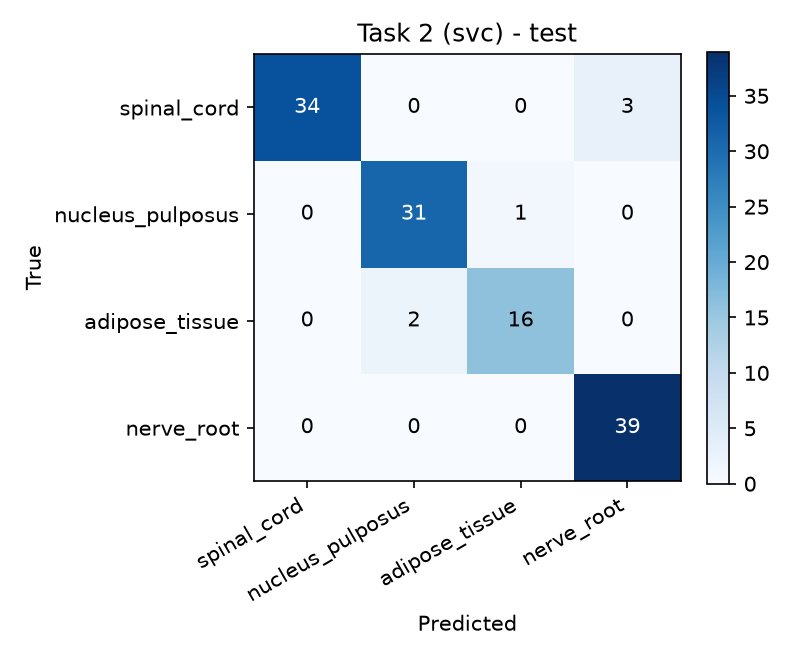
\includegraphics[width=0.46\textwidth]{../code/results/cm_task2_test.png}
\caption{Task 2 confusion matrix on the test set (sample level). Six of 126
samples are misclassified, spread over three distinct confusion pairs.}
\label{fig:cm2}
\end{figure}

The retrained SVM achieves $95.2\%$ sample-level accuracy on the test set,
slightly above its cross-validation estimate and its validation score
($94.4\%$), indicating no overfitting to the selection data. All four classes
reach F1 $\ge 0.91$; the remaining errors are three spinal-cord samples
predicted as nerve root, one nucleus-pulposus/adipose swap, and two adipose
samples predicted as nucleus pulposus.

\subsection{Aggregation Strategy Study}

\begin{table}[htbp]
\centering
\caption{Sample-level aggregation strategies for the selected SVM, same
five-fold grouped CV.}
\label{tab:agg}
\small
\begin{tabular}{lcc}
\toprule
Strategy & Sample acc. (mean) & std\\
\midrule
Majority vote (adopted) & 0.9506 & 0.0207\\
Soft voting (mean decision value) & 0.9486 & 0.0132\\
Averaged features (mean of 14 feature vectors) & 0.8971 & 0.0395\\
\bottomrule
\end{tabular}
\end{table}

Averaging the feature vectors before classification is clearly inferior
($89.7\%$) because it mixes the discriminative within-sample variation that
voting uses to cancel individual-beam noise. Soft voting matches majority
voting in the mean but has a smaller fold-to-fold spread; because the two
strategies are statistically indistinguishable here and the project
recommends majority voting, we keep majority voting as the primary protocol.

\section{Task 3: Vision Transformer}

\subsection{Provided Model (Mandatory Inference)}

The provided 1D Vision Transformer (896-point input, patch size 7,
$\dim=512$, depth 8, 10 heads, MLP width 512, dropout 0.15) was run with its
released checkpoint on the validation and test splits using the provided
inference pipeline: raw amplitudes (no Task 1 normalization, matching the
model's original training convention), softmax probabilities averaged over the
14 beams of each sample. Results are reported with the project's sample-level
metrics in Table~\ref{tab:t3res}.

\begin{table}[htbp]
\centering
\caption{Task 3 provided-ViT results (sample level).}
\label{tab:t3res}
\small
\begin{tabular}{lccccc}
\toprule
Split & Accuracy & Sensitivity & Specificity & Signal acc. & no. samples\\
\midrule
Validation & 0.9524 & 0.9524 & 0.9841 & 0.9008 & 126\\
Test & 0.9683 & 0.9683 & 0.9894 & 0.8974 & 126\\
\bottomrule
\end{tabular}
\end{table}

\begin{figure}[htbp]
\centering
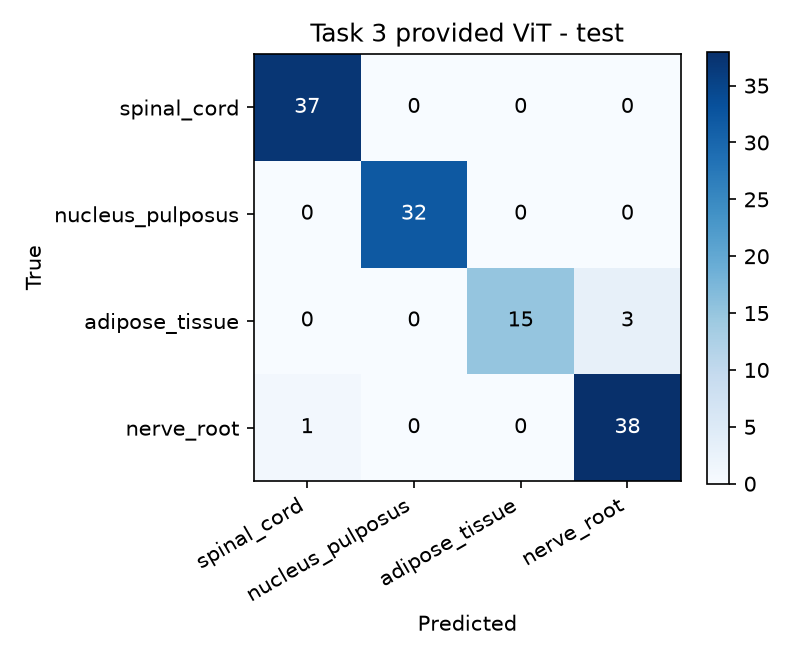
\includegraphics[width=0.46\textwidth]{../code/results/cm_task3_provided_test.png}
\caption{Task 3 provided-ViT confusion matrix on the test set (sample level).
All errors involve adipose tissue or one nerve-root sample.}
\label{fig:cm3}
\end{figure}

\textbf{Important caveat.} The dataset documentation states that the
historical training data of the provided checkpoint overlaps 88 of the 126
current validation samples and 88 of the 126 current test samples. The test
score above is therefore \emph{not} an independent generalization estimate for
this checkpoint and should be read as a diagnostic reference only. This is why
the comparison in Section~\ref{sec:comp} treats it separately from Tasks 1--2,
whose models never saw validation or test data during development.

The remaining errors are three adipose samples predicted as nerve root and one
nerve-root sample predicted as spinal cord; the same adipose/nerve-root
border seems to be the hardest region for every method in this project.

\subsection{Bonus: Independently Trained ViT}
\label{sec:bonus}

Following the bonus option, the same ViT architecture was trained from scratch
on the released training split using the provided training script
(\texttt{train\_minimal.py}) and its default configuration
(Table~\ref{tab:bonuscfg}). The training set was used for fitting, the
validation set for model selection (the best epoch by validation sample
accuracy was kept), and the test set was evaluated exactly once after training
finished; no test label participated in any training or selection decision.

\begin{table}[htbp]
\centering
\caption{Bonus ViT training configuration (provided script defaults).}
\label{tab:bonuscfg}
\small
\begin{tabular}{ll}
\toprule
Item & Value\\
\midrule
Input & raw amplitudes (same convention as the provided model)\\
Architecture & patch 7, dim 512, depth 8, heads 10, MLP 512, dropout 0.15\\
Optimizer & AdamW, lr $3\times10^{-4}$\\
Batch size / epochs & 64 signals / 20\\
Model selection & best validation sample accuracy (epoch 14)\\
Data use & train: fitting; validation: selection; test: final evaluation only\\
\bottomrule
\end{tabular}
\end{table}

\begin{table}[htbp]
\centering
\caption{Bonus ViT results with the project's sample-level metrics; the
provided checkpoint is repeated for reference.}
\label{tab:bonusres}
\small
\begin{tabular}{llccc}
\toprule
Model & Split & Accuracy & Sensitivity & Specificity\\
\midrule
Student ViT (clean, this work) & Validation & 0.9841 & 0.9841 & 0.9947\\
Student ViT (clean, this work) & Test & 0.9683 & 0.9683 & 0.9894\\
Provided ViT (overlap caveat) & Validation & 0.9524 & 0.9524 & 0.9841\\
Provided ViT (overlap caveat) & Test & 0.9683 & 0.9683 & 0.9894\\
\bottomrule
\end{tabular}
\end{table}

The independently trained model matches the provided checkpoint on the test
set ($96.8\%$) and surpasses it on validation ($98.4\%$). Because 88 of 126
test samples were part of the provided checkpoint's historical training data,
the student model's $96.8\%$ is the more trustworthy estimate of true
generalization at this accuracy level. Its per-class test metrics
(Table~\ref{tab:bonusper}) again show adipose tissue as the weakest class
(F1 $0.944$); the two remaining errors are one adipose sample predicted as
spinal cord and two nerve-root samples predicted as spinal cord.

\begin{table}[htbp]
\centering
\caption{Student ViT per-class test metrics (one-versus-rest).}
\label{tab:bonusper}
\small
\begin{tabular}{lccccc}
\toprule
Class & Precision & Recall & Specificity & F1 & Support\\
\midrule
Spinal cord & 0.923 & 0.973 & 0.966 & 0.947 & 37\\
Nucleus pulposus & 1.000 & 1.000 & 1.000 & 1.000 & 32\\
Adipose tissue & 0.944 & 0.944 & 0.991 & 0.944 & 18\\
Nerve root & 1.000 & 0.949 & 1.000 & 0.974 & 39\\
\bottomrule
\end{tabular}
\end{table}

\subsection{Comparison of Methods}
\label{sec:comp}

\begin{table}[htbp]
\centering
\caption{Test-set comparison (sample level, majority/soft voting).}
\label{tab:comp}
\small
\begin{tabular}{lccc}
\toprule
Method & Accuracy & Sensitivity & Specificity\\
\midrule
Task 1: interpretable statistical rule (depth-5 tree) & 0.8333 & 0.8333 & 0.9444\\
Task 2: SVM RBF ($C=100$) on DWT features & 0.9524 & 0.9524 & 0.9841\\
Task 3: provided ViT (overlap caveat) & 0.9683 & 0.9683 & 0.9894\\
Task 3 (bonus): independently trained ViT & 0.9683 & 0.9683 & 0.9894\\
\bottomrule
\end{tabular}
\end{table}

The ViT benefits from learning its own time-domain representation and achieves
the highest signal-level accuracy ($89.7\%$ vs $80.4\%$ for the SVM), so fewer
errors have to be repaired by voting. Given the overlap caveat, however, the
honest conclusion is that the tuned classical pipeline (Task 2) is on par with
the provided deep model, while being far cheaper and fully interpretable up to
the decision rule.

\section{Discussion}

\textbf{Performance across tissue types.} Adipose tissue is consistently the
hardest class (F1 $0.56$/$0.91$/$0.91$ in Tasks 1/2/3) and is the source of
most residual errors. Two factors explain this: it has the fewest samples
(73/18/18), and its ultrasound signature overlaps with the surrounding
nucleus pulposus and nerve root. Nerve root is the easiest class, separated
mainly by its low detail-band kurtosis. The gap between signal-level
($\approx 67$--$90\%$) and sample-level ($83$--$97\%$) accuracy is large for
all methods, which shows that within-sample noise, not systematic tissue
confusion, is the dominant error source; majority voting removes most of it.

\textbf{Effectiveness of the features.} Detail-band statistics at the two
finest scales (cD1/cD2) carry most of the discriminative information
($F$-scores an order of magnitude above smooth-band features), consistent with
the interpretation that tissue boundaries and scatterer spacing shape the
high-frequency content of the echo. Six statistics per DWT component proved
sufficient for $95\%$ sample accuracy with an SVM, without any hand-crafted
time-domain features. The fixed DWT basis may, however, fit some samples
poorly; EWT's adaptive bands or VMD modes are natural next steps.

\textbf{Limitations.} (i) The provided-ViT score is contaminated by the
train/test overlap documented in the dataset; the independently trained ViT
(Section~\ref{sec:bonus}) removes this caveat and reaches the same test
accuracy ($96.8\%$), so the deep-learning advantage over the tuned SVM
($95.2\%$) is real but small. (ii) The
statistical rule, although explicit, is a depth-5 tree trained on a 36-feature
space; with few adipose samples it sacrifices that class. (iii) All results
come from single splits; only CV stds quantify variability. (iv) The weak
class is small, so per-class metrics for adipose tissue carry large
uncertainty ($\pm$ a few samples). \textbf{Potential improvements} include
EWT-based adaptive features, cost-sensitive thresholds for adipose tissue,
ensemble/stacked classifiers, attention-based beam aggregation instead of
voting, and fine-tuning the ViT on the released training split only
(Section~\ref{sec:bonus}).

\section{Conclusion}

We built a complete spinal-tissue classification pipeline on 14-beam
ultrasound samples. DWT (db4, level 5) statistical features with an SVM give
$95.2\%$ sample-level test accuracy under a strictly leak-free protocol; an
explicit threshold rule reaches $83.3\%$ while remaining fully interpretable;
the provided ViT reports $96.8\%$ but with a train/test overlap caveat that
prevents treating it as an independent estimate. An independently trained ViT
reproduces $96.8\%$ test accuracy ($98.4\%$ validation) without any overlap,
confirming that deep and classical models perform comparably on this dataset. Sample-level majority voting
is essential, contributing roughly 15 accuracy points over signal-level
predictions.

\appendix

\section{Metric Definitions}
\label{app:metrics}

All metrics are computed at the sample level with one-versus-rest (OvR)
per-class counts and micro aggregation as specified in the project:
$\mathrm{TP}_{\mathrm{micro}}=\sum_c \mathrm{TP}_c$, etc., then
accuracy $=(TP+TN)/(TP+TN+FP+FN)$, sensitivity $=TP/(TP+FN)$, and
specificity $=TN/(TN+FP)$.
For single-label multi-class problems $TP_{\mathrm{micro}}/(TP_{\mathrm{micro}}+FP_{\mathrm{micro}})
= TP/(TP+FN) =$ overall accuracy, so the reported accuracy equals the
micro-averaged sensitivity. For reference, the literal formula applied to OvR
micro sums gives $(TP_{\mathrm{micro}}+TN_{\mathrm{micro}})/(\dots) = (1+\text{accuracy})/2$
because each correctly classified sample is a true negative for the $C-1$
other classes; our tables report the standard overall accuracy
(as ``overall classification correctness'') together with the micro
sensitivity and specificity.

\section{Full Statistical Rule}
\label{app:rule}

The following is the exact exported rule selected in Task 1
(\texttt{results/task1\_rule.txt}); a feature test evaluates true when the
feature value is \emph{less than or equal to} the threshold.

\lstinputlisting[basicstyle=\ttfamily\scriptsize, frame=single, numbers=left, numberstyle=\tiny]{../code/results/task1_rule.txt}

\section{Reproducibility}

All experiments used Python 3.14 with numpy 2.5, SciPy 1.18,
scikit-learn 1.9, PyWavelets 1.8, and PyTorch 2.14 (CUDA). Fixed seeds: 42
(feature/ML pipeline) and the released split seed 20260907. Running
\texttt{bash run\_all.sh} inside \texttt{code/} reproduces every number and
figure in this report and writes them to \texttt{code/results/}. The test
set was touched only by the final evaluation commands of each task after all
hyperparameters and rules were frozen; no test label influenced any design
choice.

\end{document}
